\documentclass[binding=0.7cm, oneside]{sapthesis}

\usepackage{microtype}
\usepackage{hyperref}
\usepackage {subcaption}
\usepackage{enumitem}
\hypersetup{pdftitle={My thesis},pdfauthor={Francesco Danese}}

\title{A Robust Person Identification Method Through Wi-Fi Signals}
\author{Francesco Danese}
\IDnumber{1926188}
\course{Applied Computer Science and Artificial Intelligence}
\courseorganizer{Faculty of Information Engineering, Informatics, and Statistics}
\AcademicYear{2022/2023}
\advisor{Prof. Luigi Cinque}
\coadvisor{Prof. Danilo Avola}
\coadvisor{Prof. Daniele Pannone}
\copyyear{2023}
\authoremail{francescodanese01@gmail.com}
\begin{document}
\frontmatter
\maketitle

\begin{abstract}
    This thesis deals with myself.
\end{abstract}

\tableofcontents
\mainmatter
\chapter{Introduction}
In the last years, Wi-Fi technology is turning into a ubiquitous and fundamental tool, not only for providing
constant and easy-access internet connection but also for enabling the development of the Internet of Things and
radio-based sensing applications. Cutting-edge Wi-Fi sensing systems use wireless signals to detect events or changes,
such as motion and gesture recognition \cite{gesture_recognition}, in the permeated environment leveraging the disturbances
and variations in the received radio signal. In this work, Wi-Fi sensing technology is employed for person Identification, a task
usually achieved by vision-based systems through the use of RGB cameras. In common scenarios, person Identification is a classification
task where the input features, such as an image or a video of a particular individual, is examined in order to recognize him among a specific
set of people. To reach this goal, in modern approaches the raw input image is analyzed in order to model a person appearance and physical
constitution, by extracting some key features that will be use for inference, as shown in Fig. \ref{fig:visionID}. State-of-the-art methods include leveraging deep learning models
trained to identify a human, like: Convolutional Neural Network for detecting the face of the person \cite{cnn_face_id} and recognize him;
Recurrent Neural Networks \cite{Recurrent_nn_reid} and their variants, such as LSTMs, for working with sequences of data like video sequences
and exploiting the unique person behavior like the walking gait \cite{Gait_cnn}; Attention mechanisms, as seen in models like Transformers \cite{Transformers_reid},
for their ability to focus on relevant parts of an image or sequence therefore locating the discriminative features.
Although vision-based methods have achieved remarkable results, several issues arise during real-world scenarios, including:
subject occlusion and pose; different viewing angles and image scale; ambient changes in illumination; modifications in personal look
(clothes, haircut, glasses) and privacy concerns due to the sensitive nature of personal imaging data. To address these challenges,
a non-conventional approach can be adopted, that walks away from images and vision avoiding the aforementioned issues, through the use of
completely different types of data: Wi-Fi signals.
\begin{figure}[h!]
    \centering
    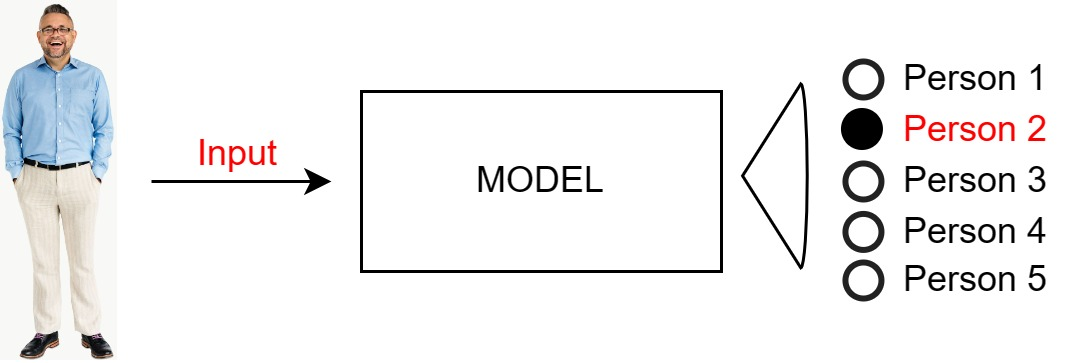
\includegraphics[scale=0.3]{images/Person_id.jpg}
    \caption{Image-based person ID within a group of 5 people.}
    \label{fig:visionID}
\end{figure}

Wi-Fi technology has revolutionized the way we connect and communicate in the digital age. It enables wireless communication between devices by
utilizing radio signals transmitted by access points (APs). The signals can be influenced by various factors, such as objects and people,
leading to signal variations along their path. These variations, essential for understanding the wireless environment,
are captured through measurements like the Received Signal Strength Indicator (RSSI) and Channel State Information (CSI),
which play a pivotal role in implementing wireless sensing applications. The RSSI serves as a measure of the reduction in the strength of radio signals
as they travel through space, capturing the way signals diminish over distance. Even though this metric has found widespread utilization within numerous
indoor localization systems \cite{RSSI_indoorloc,RSSI_indoorloc_new}, which goal is to find where a certain target is in an enclosed location with meter-precision,
it experiences unsustainable performance drops in complex situations, due to several limitations. The problems associated with RSSI stem from its simplicity and
lack of granularity, which restrict its ability to capture detailed signal characteristics and changes accurately. In fact, for a given wireless data packet, RSSI
provides a single value computed at MAC layer, that represents the overall signal strength, without differentiating between the effects of multipath interference,
signal reflections, or other external factors. Moreover, the relationship between RSSI values and the real signal strength is often non-linear, so that small changes
in RSSI may not correspond to proportional changes in signal strength, making it challenging to interpret signal variations accurately. For these relevant reasons, RSSI fails
to provide detailed insights into how the signal interacts with the surrounding environment \cite{RSSI_reliability_indoorloc}. On the other hand, the CSI is derived
from the PHY layer's orthogonal frequency-division multiplexing (OFDM) transmission technology and includes detailed signal information defined at the subcarrier level,
making it more stable and capable of carrying a higher level of signal information. CSI measurements offer access to a broader range of signal properties, including
amplitude and phase for each subcarrier, providing higher granularity than RSSI \cite{CSI_RSSI}. Furthermore, CSI can be computed using commodity Wi-Fi devices,
making it a popular choice in Wireless sensing applications. To ensure the quality of received CSI measurements, signal pre-processing techniques are often employed,
such as removing amplitude outliers and phase offsets, and machine learning or deep learning approaches are subsequently applied to address the specific final task.

Ultimately, previous investigations on electromagnetic waves interactions with biological tissues \cite{tissues_waves_interaction} have revealed that signal propagation around a human body is
highly dependent on biometric characteristics, such as body structure, weight, height, skin and tissues composition, with a great variability among different individuals.
The aim of this work is then to harness the biological-related radio signals fluctuations, captured by CSI, that occur in a WiFi-pervaded environment when a person is present, and extract
important insights to enable the person Identification.

\chapter{The Wireless Channel}
This section introduces the theoretical concepts related to the wireless communication channel, that are necessary to grasp the foundational technology behind Wi-Fi sensing applications, such as Human Identification

\section{Electromagnetic Waves}
The fundamental characteristic of all wireless communications, including Wi-Fi transmission, is the use of Electromagnetic (EM) radiation to carry information,
encapsulating data in the form of EM waves. In a vacuum, electromagnetic waves travel at the speed of light (around 299 792 km/s) denoted by the letter $c$.
When passing through a material medium, they are slowed depending on the medium's permeability and permittivity but the air in the Earth's atmosphere is thin enough that EM waves
travel very close to the speed of light. Each wave is produced by a transmitting antenna (TX) that generates synchronous oscillations between electric and magnetic fields,
and it is characterized by several properties, shown in Fig. \ref{fig:wave}: The wavelength, measured in meters, which is the distance between consecutive corresponding points of the same phase on the wave, such as
two adjacent crests (the highest points), troughs (the lowest points), or zero crossings; The amplitude, in meters, that is the distance from the resting position to
the maximum displacement of the wave; The frequency, measured in Hertz (Hz), that is the number of oscillation cycles per second or
how many crests (or troughs) pass a location in a certain amount of time. The frequency is equal to $1/p$, where $p$ is the period of the wave, which is the time in seconds that the signal takes
to return to the equilibrium position, starting from the previous one (also called a full "cycle").
\begin{figure}[h!]
    \centering
    \begin{subfigure}{0.48\textwidth}
        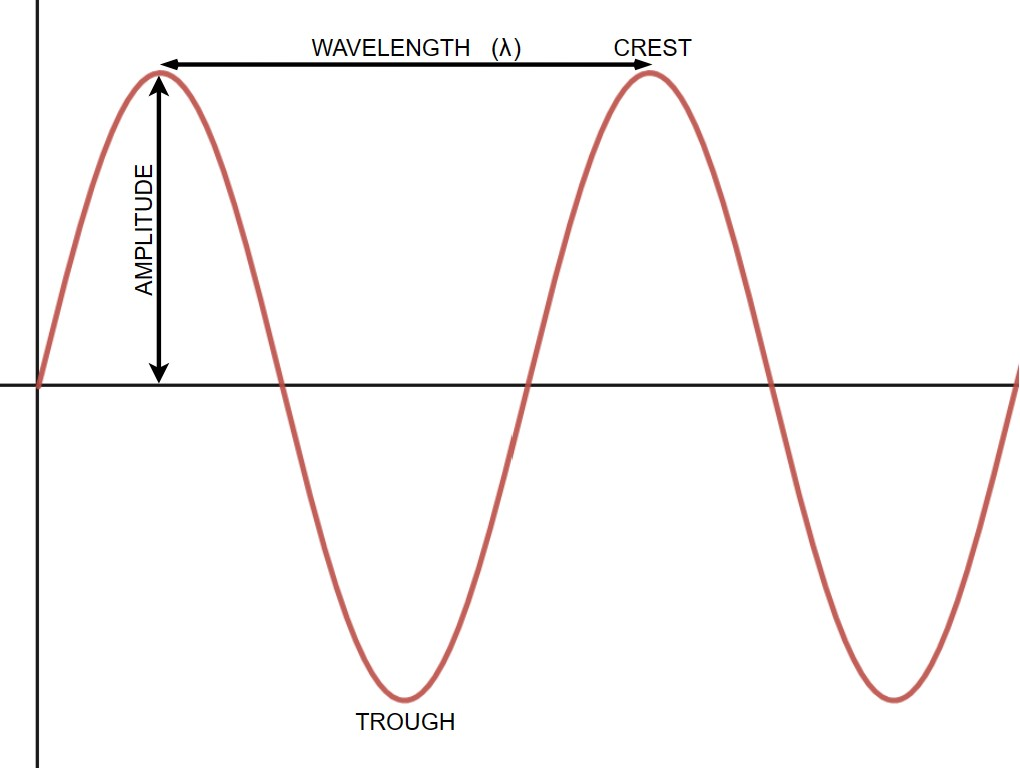
\includegraphics[width=\textwidth]{images/wave.jpg}
        \caption{Representation of a wave’s properties}
        \label{fig:wave}
    \end{subfigure}
    \hfill
    \begin{subfigure}{0.48\textwidth}
        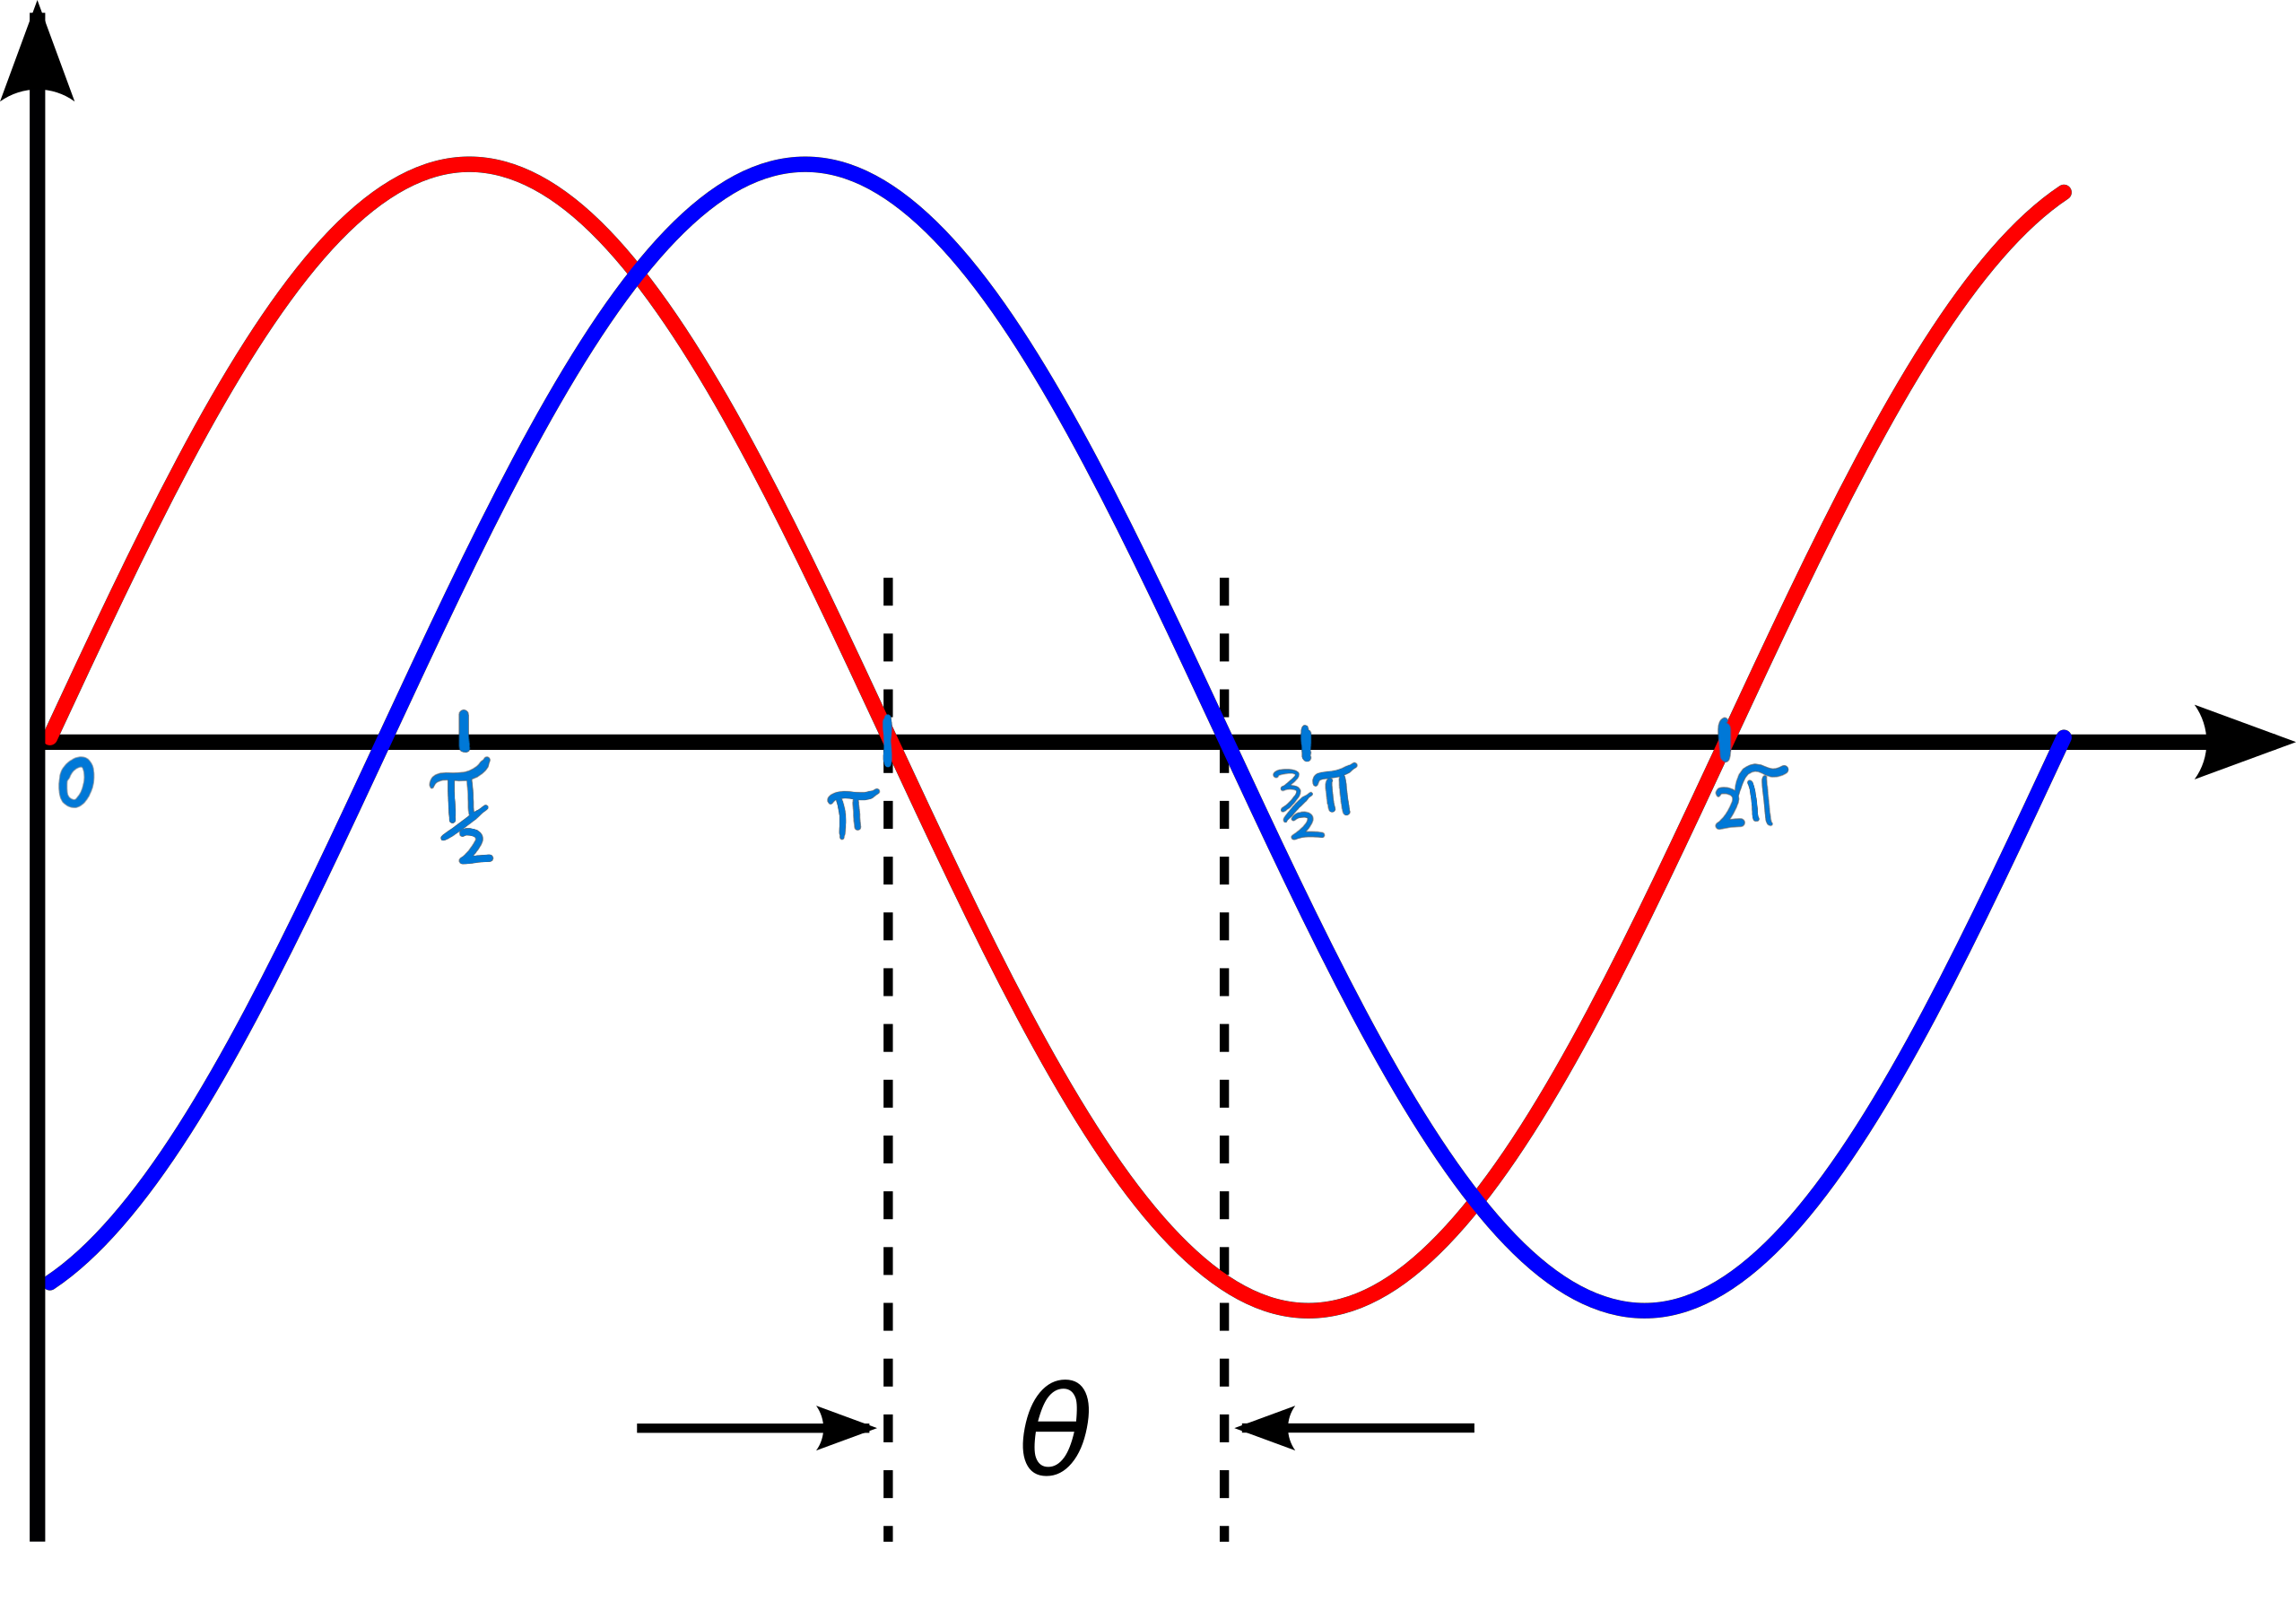
\includegraphics[width=\textwidth]{images/Phase_shift2.png}
        \caption{Illustration of a phase shift.}
        \label{fig:phase}
    \end{subfigure}
\end{figure}
The mathematical link between the frequency $f$, the wavelength $\lambda$, and the
wave propagation velocity $v$ is expressed as follows:
$$ f = \frac{v}{\lambda} $$
Where in vacuum $v = c$, the speed of light, as explained before. From the previous equation we get:
$$ v = f\lambda \qquad and \qquad \lambda = \frac{v}{f} $$
indicating how the frequency and wavelength of an EM wave are directly proportional to the propagation velocity and inversely proportional to each other.

The last key component used to describe a wave is the phase. The phase of a wave refers to its position within one complete cycle, describing how much of
the cycle has occurred at a specific point in space and time. It is often measured in radians or degrees, and it helps determine where a wave is in its
oscillation at a given moment. A phase angle of 0 represents the starting point of a cycle, while $2\pi$ (or 360°) corresponds to one complete cycle.
When comparing two waves, the phase difference, or phase shift, is the angular difference between their phase angles, and it indicates how "out of sync"
or "in sync" they are, as seen in Fig. \ref{fig:phase}. Considering two sinusoidal waves, when the phase difference is a multiple of $2\pi$, the addition
of the two waves results in a constructive interference, leading to reinforcement and a larger amplitude. Vice versa, destructive interference occurs when
the phase difference is an odd multiple of $\pi$, leading to cancellation and a smaller amplitude.

With those characteristic we can formulate the mathematical representation of a periodic wave, that tells us the momentary amplitude at instant $t$:
$$ a(t) = A\cos(2\pi ft + \phi) $$
made up of the following components:
\begin{itemize}[itemsep=1.5pt]
    \item $a(t)$: The instantaneous amplitude of the wave at time t.
    \item $A$: The amplitude of the wave, its maximum value.
    \item $2\pi f$: The angular frequency in $rad/s$, where $f$ is the frequency in Hertz ($1/s$)
    \item $t$: The time in seconds, indicating the instant at which you evaluate $a(t)$
    \item $\phi$: The phase offset, in radians, that determines the wave' starting position.
\end{itemize}
When $\phi$ is non-zero, the entire waveform appears to be shifted in time by $\frac{\phi}{2\pi f}$ seconds. A negative value represents a delay,
and a positive value represents an advance. The above equation describes a sinusoidal wave as a function of time, and it's a fundamental building
block in understanding and modeling periodic oscillations and waveforms in various fields of science.
\section{I/Q sampling}
\label{sec:IQ}
In many real-world applications, information is transmitted through analog signals, which vary continuously over time. To process and analyze these signals
using digital electronics, they need to be converted into a discrete digital form, a process known as sampling. I/Q sampling is a method used to sample
and represent a complex-valued analog signal, from which we can retrieve both amplitude and phase information. The "I" component represents the in-phase
or real part of the signal, while the "Q" component represents the quadrature or imaginary part of the signal. Denoting with $A$ the amplitude and with
$\phi_t$ the phase of the wave at instant $t$, we got:
$$ I(t) = A\cos(\phi_t) \qquad and \qquad Q(t) = A\sin(\phi_t)$$
Now, we can construct the complex number at any given time $t$ by combining the "I" and "Q" components
$$Z(t) = I(t) + jQ(t)$$
Where $j$ is the imaginary unit ($j^2 = -1$). Therefore, as depicted in Fig. \ref{fig:IQ_sample}, any sinusoidal wave can be
described by a composition of those two components (that is, by a single complex number), from which it is possible
to obtain the amplitude and the phase using the following equations:
$$ A = \sqrt{I(t)^2 + Q(t)^2} \qquad and \qquad \phi_t = atan2(I(t), Q(t)) $$
The first formula is simply the Pythagorean theorem applied to the two sides, in our case I and Q, to find the hypotenuse, that matches the amplitude.
The second one uses $atan2(x,y)$, a function that returns the angle formed by any vector [x, y] with the positive x-axis, bounded in the interval ($-\pi$, $\pi$].
The angle is positive if counterclockwise, negative if clockwise. Additionally, since $\cos(x) + j\sin(x) = e^{jx}$, we can represent the I/Q sample in the Euler's form:
$$Z(t) = A(\cos(\phi_t) + j\sin(\phi_t)) = Ae^{j\phi_t}$$
\begin{figure}[h]
    \centering
    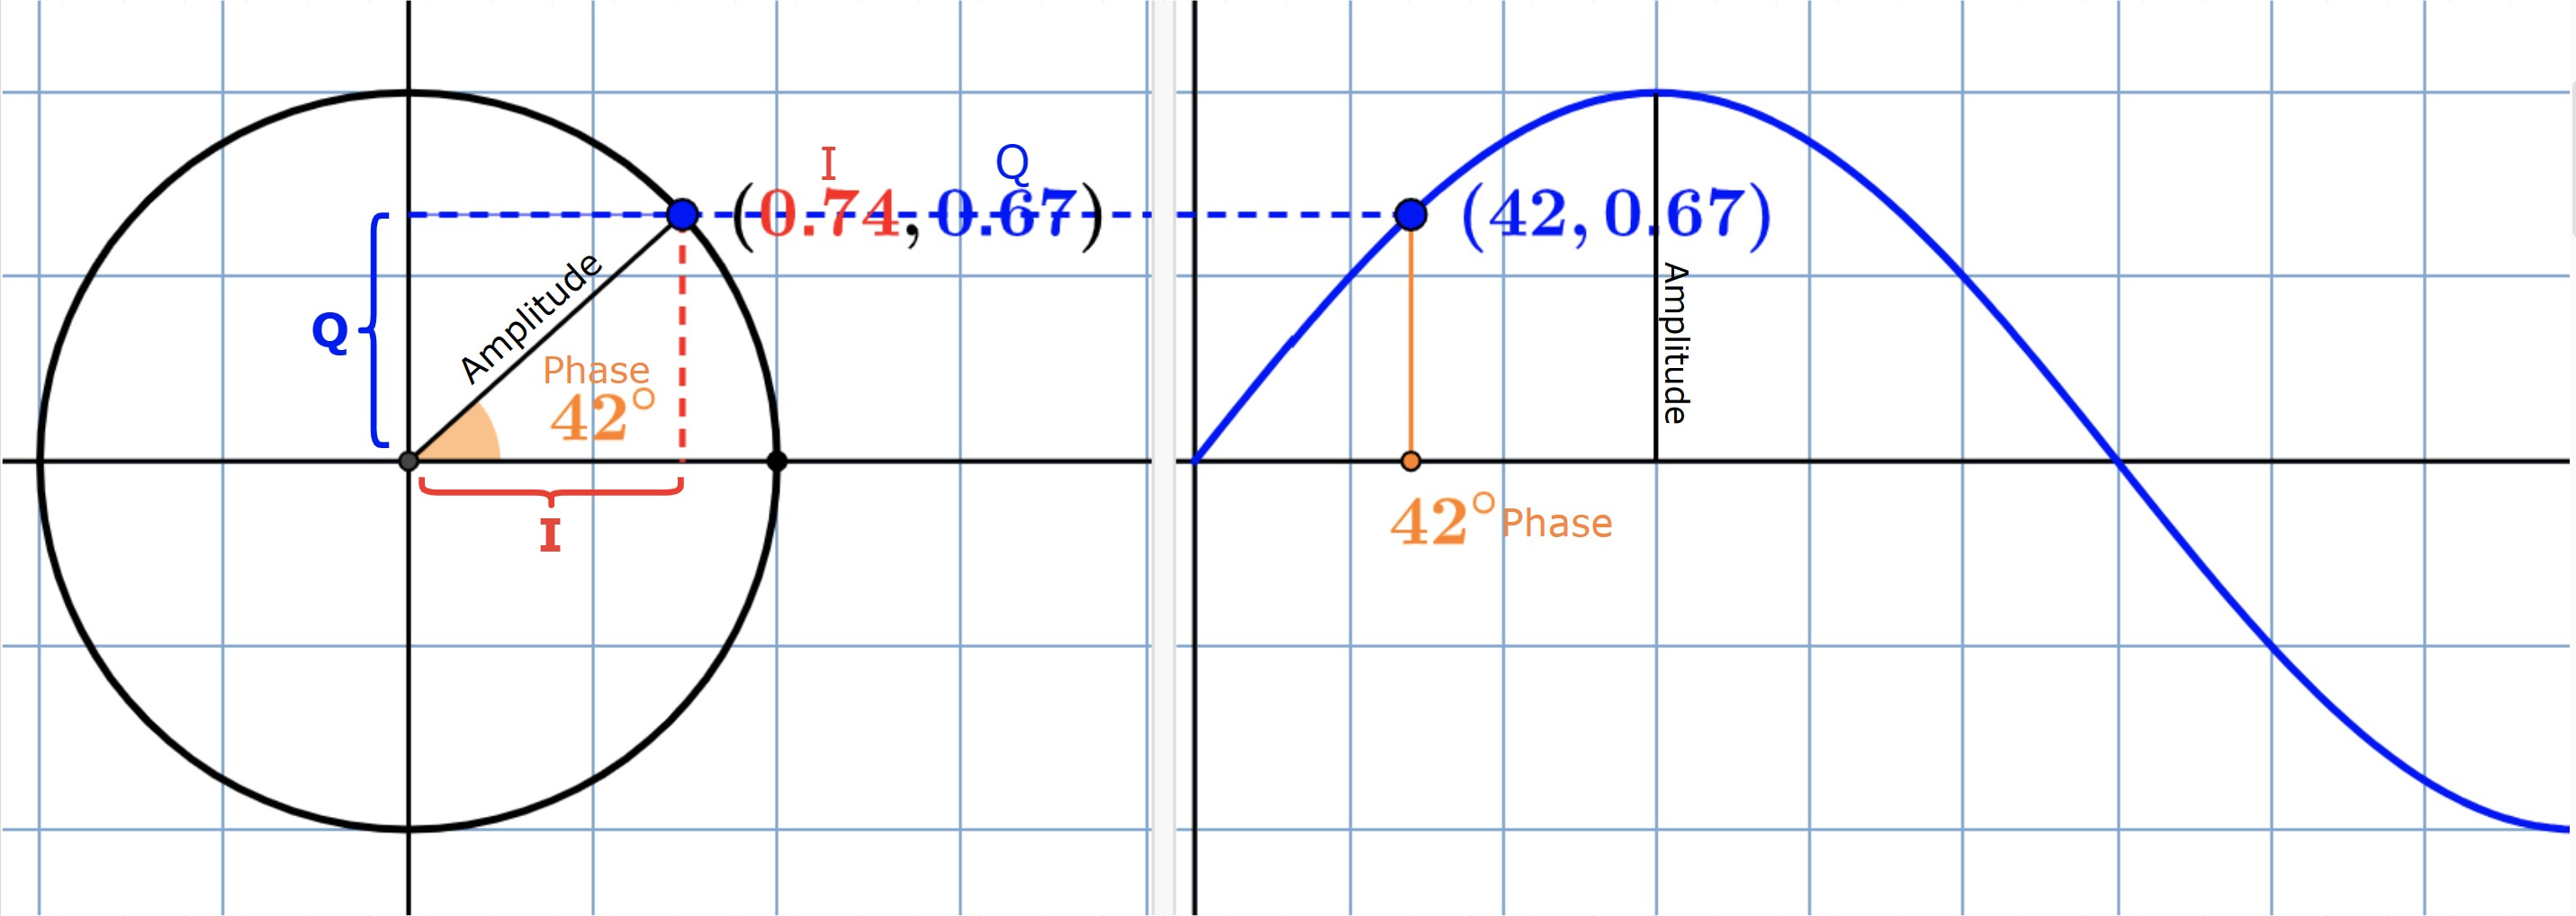
\includegraphics[width=0.96\textwidth]{images/IQ_sampling.jpg}
    \caption{Decomposition of a wave in I/Q components.}
    \label{fig:IQ_sample}
\end{figure}

\section{Orthogonal Frequency-Division Multiplexing}
Orthogonal frequency-division multiplexing (OFDM) is a modulation scheme used in wireless communication systems such as 802.11n
which encodes data streams into multiple overlapping subcarrier frequencies. In a traditional single-channel modulation scheme,
each data bit is sent serially or sequentially one after another. With OFDM a single information stream is split among several
closely spaced narrowband subchannel frequencies instead of a single Wideband channel \cite{OFDM_basics}. This enables each substream's
data rate to be lower than would be required by a single stream of similar bandwidth and makes the system less susceptible to corruption.
Even though the subchannel frequencies are closely spaced and do overlap to a degree,
they remain orthogonal, maintaining their distinct separation due to meticulous selection.
This strategy ensures that any interference is effectively negated.

OFDM signals are modelled in the frequency domain as the $sinc$ function:
$$sinc(f) = \frac{\sin(f)}{f}$$
The $sinc$ function has a central peak at zero frequency and then oscillates symmetrically around zero. It is characterized by its main lobe,
which contains most of its energy, and smaller side lobes that decrease in amplitude as you move away from the central peak, as seen in Fig.
\ref{fig:sinc_func}. The choice of the $sinc$ function is made due to its property of enabling orthogonal placement of each subcarrier with
respect to the others \cite{EdgeWiFiSensing2022}, as illustrated in Fig. \ref{fig:multiple_sinc} where five $sinc$ functions are strategically
positioned so that the primary subcarrier frequency (one is marked in red) coincides with a frequency at which all accompanying $sinc$ functions
assume a value of zero. This orthogonal configuration ensures that the summation of all five selected subcarriers maintains its peak values,
as presented in Fig. \ref{fig:summation}.
\begin{figure}[h!]
    \centering
    \begin{subfigure}{0.45\textwidth}
        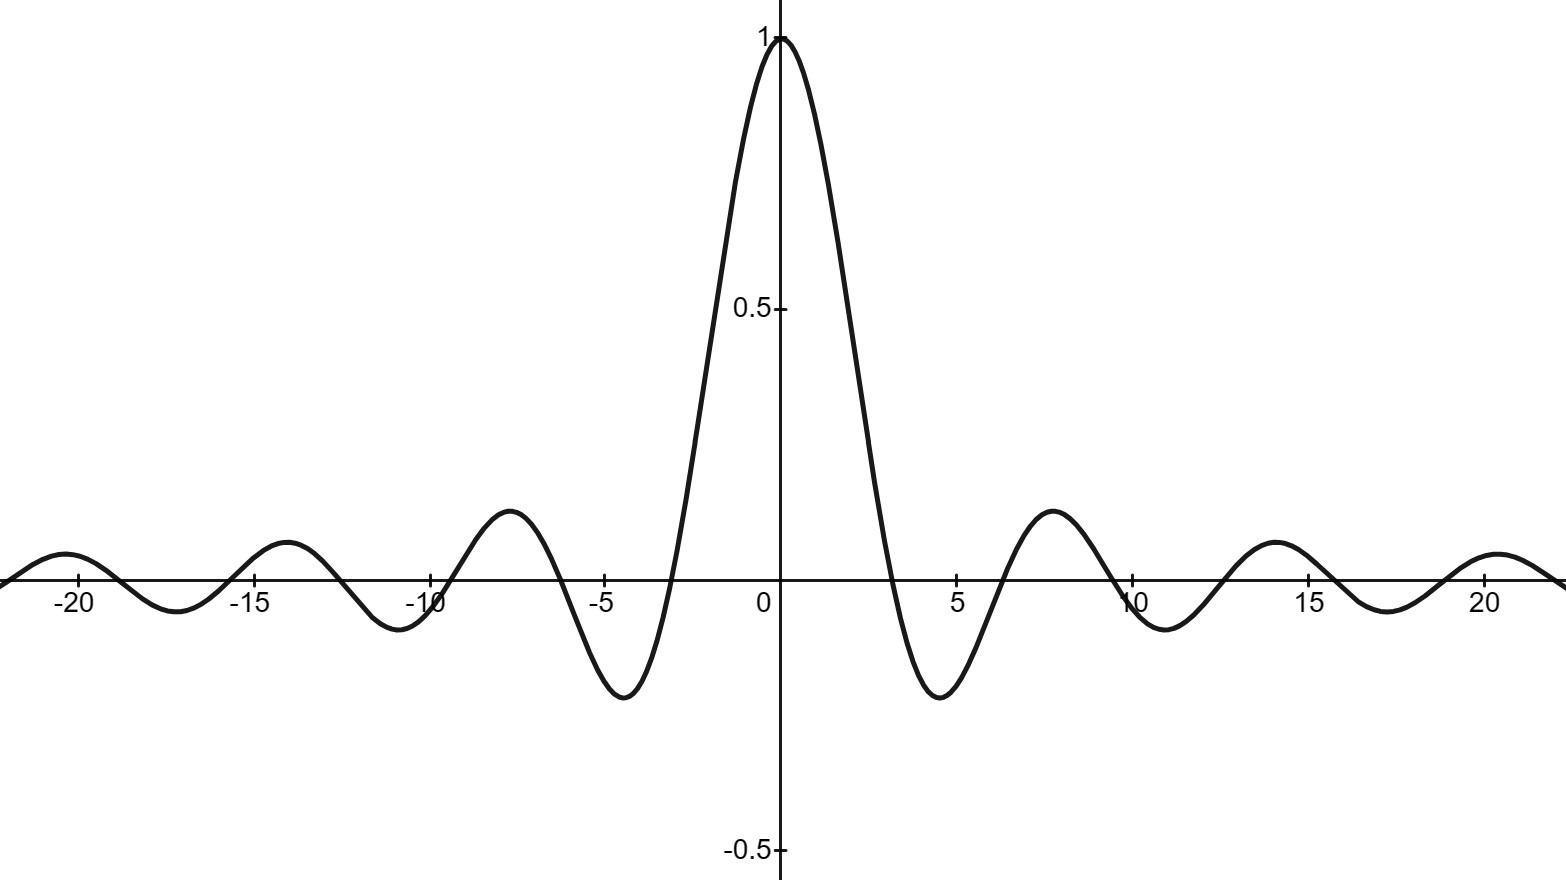
\includegraphics[width=\textwidth]{images/sinc_func_alone.jpg}
        \caption{The $sinc$ function for a single subcarrier signal.}
        \label{fig:sinc_func}
    \end{subfigure}
    \quad
    \begin{subfigure}{0.45\textwidth}
        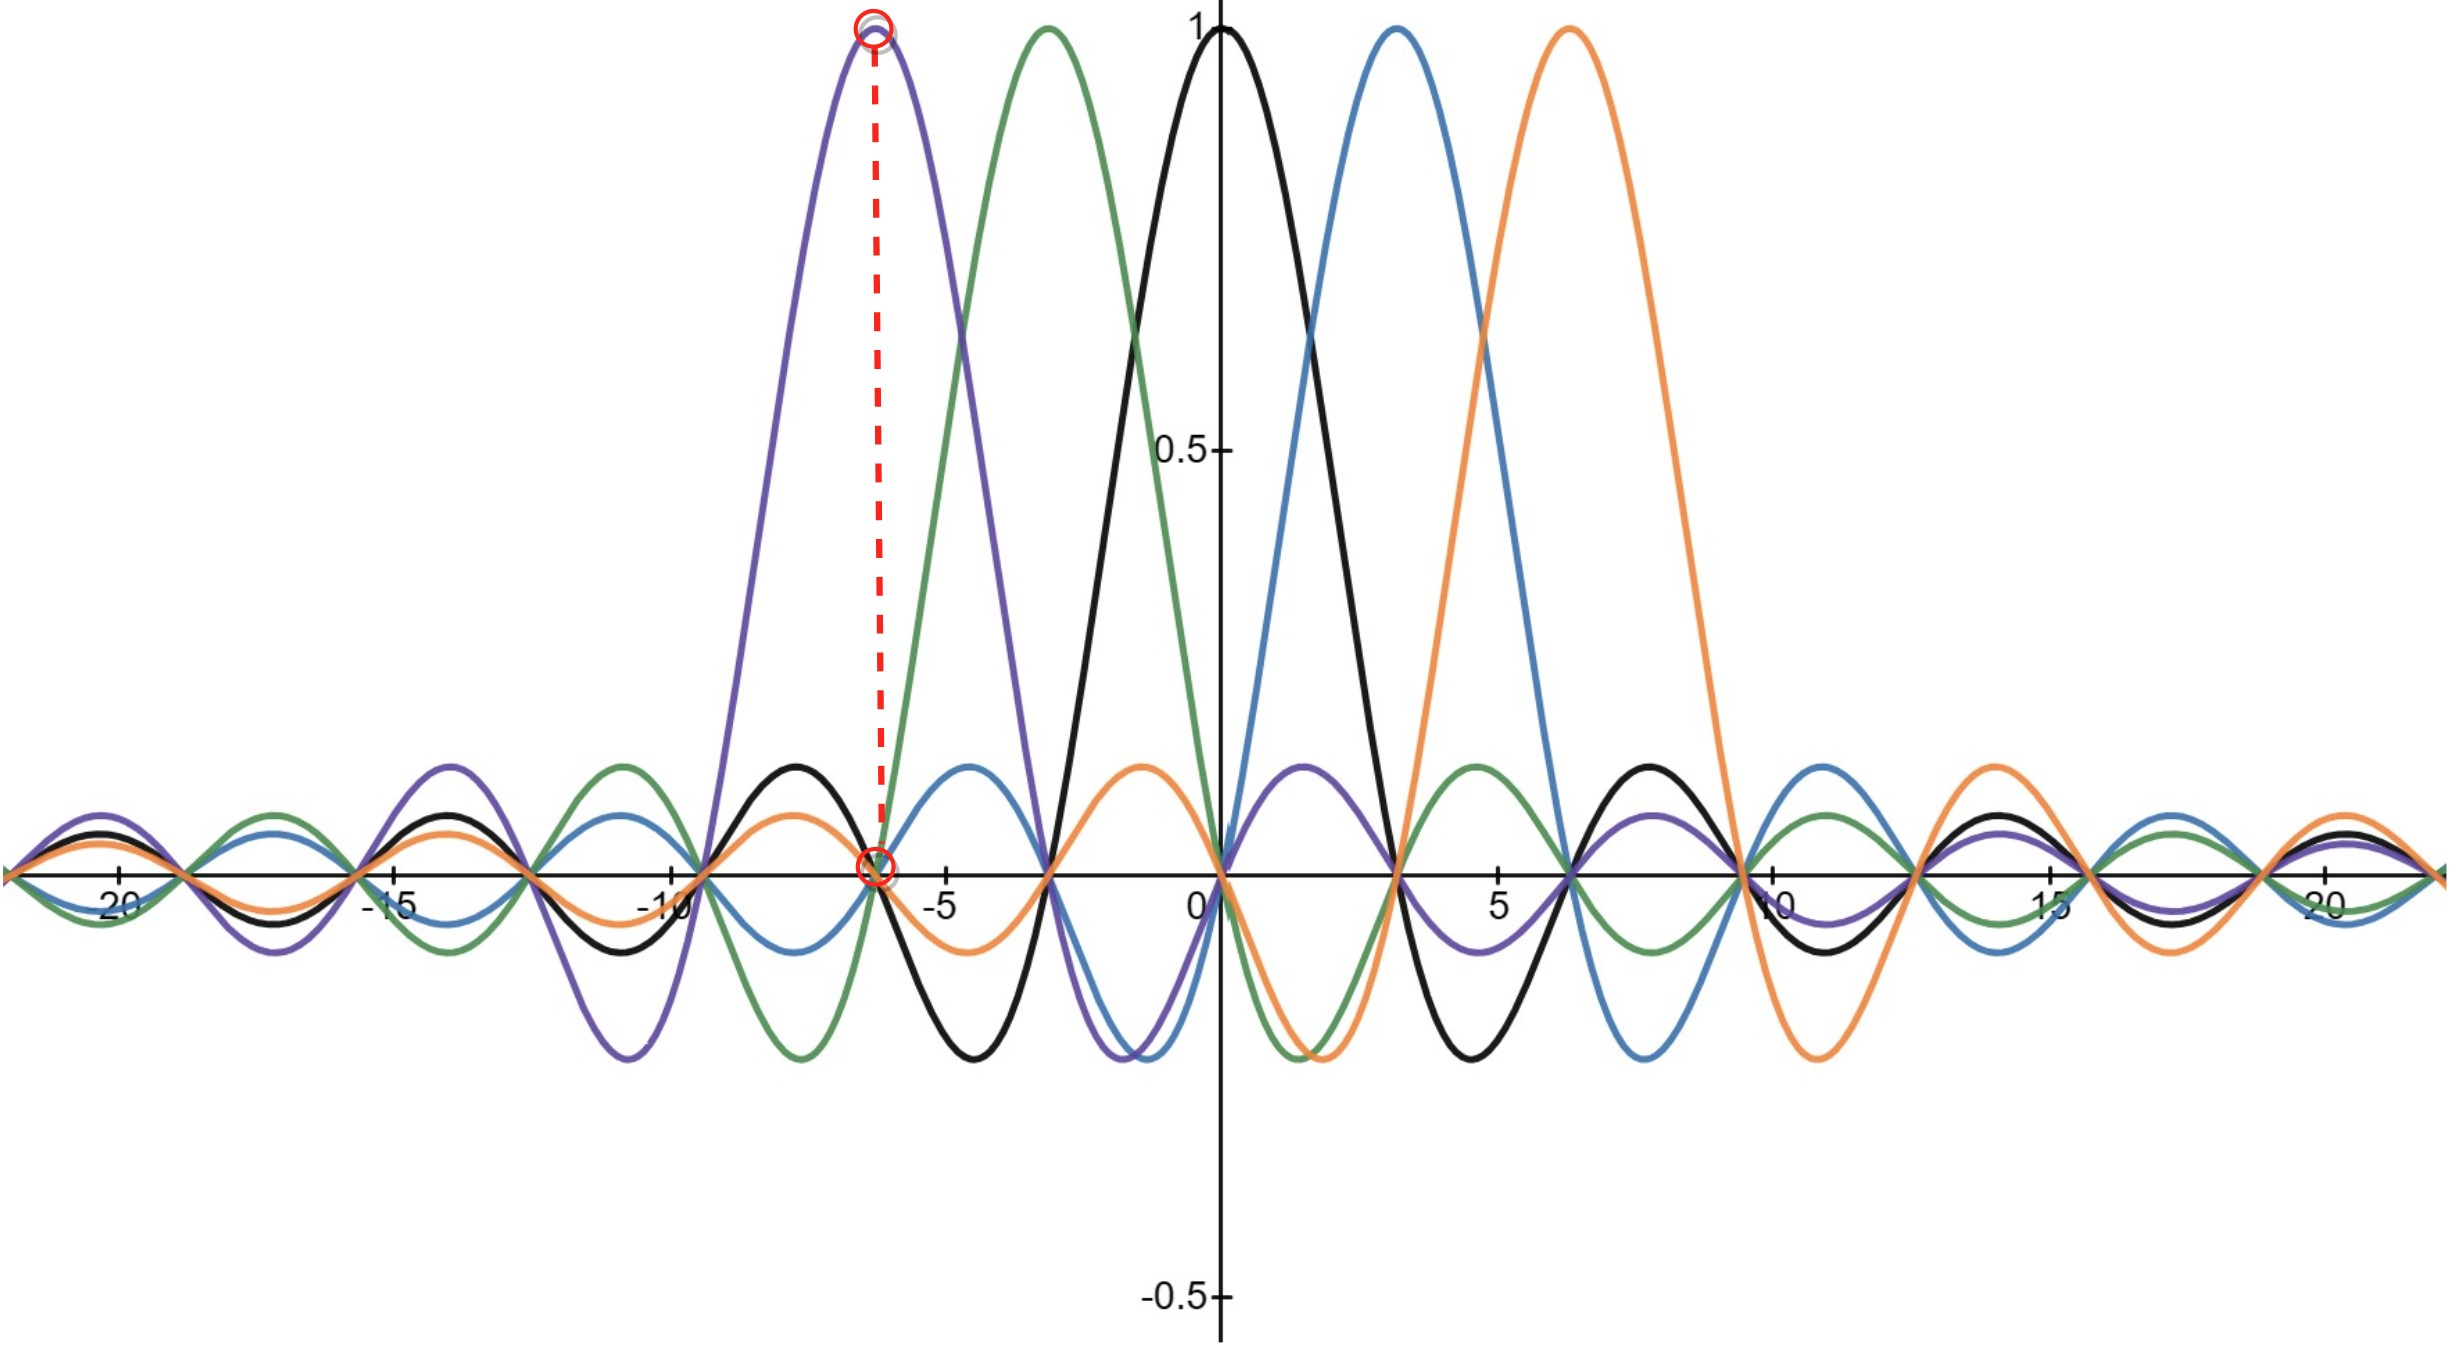
\includegraphics[width=\textwidth]{images/multiple_sinc.jpg}
        \caption{Orthogonal $sinc$ functions for multiple subcarriers.}
        \label{fig:multiple_sinc}
    \end{subfigure}
    \begin{subfigure}{0.45\textwidth}
        \centering
        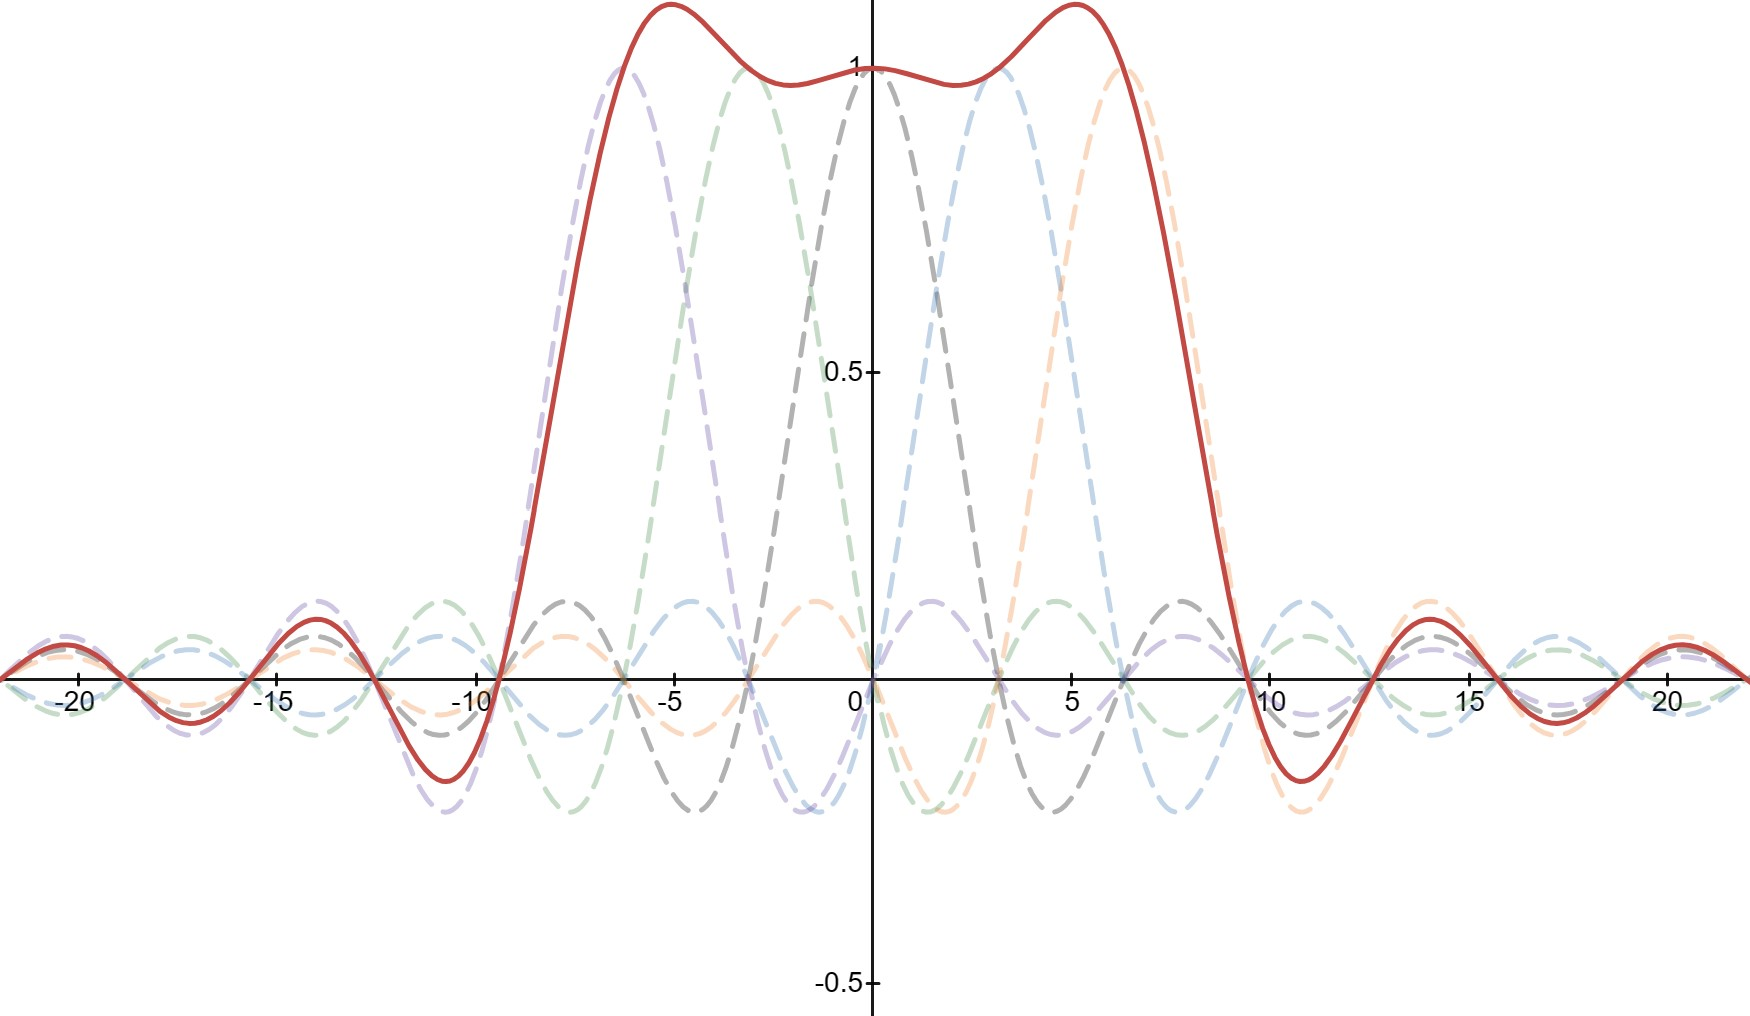
\includegraphics[width=\textwidth]{images/summationSinc.jpg}
        \caption{Signals summation.}
        \label{fig:summation}
    \end{subfigure}
\end{figure}

In order to transmit bits, a signal undergoes modulation. In wireless communication, modulation is the process of altering one or more characteristics
of a periodic waveform, called the carrier signal, with a separate signal called the modulation signal that typically contains information to be transmitted.
With OFDM, each subcarrier represents a single digital symbol that is being transmitted and can be modulated through various methods \cite{modulations} such
as Amplitude Shift Keying (ASK), Binary Phase-Shift Keying (BPSK) or Quadrature Amplitude Modulation (QAM). ASK involves switching the amplitude of the carrier
signal between two different levels (high and low) to represent binary data while BPSK achieves the same thing by altering the phase (usually $0^\circ$ and $180^\circ$)
to represent the travelling bits. QAM, widely used in Wi-Fi communication systems, combines instead both amplitude and phase modulation to convey multiple bits
of digital information in each modulation symbol, resulting in a higher data rate. Every OFDM symbol encodes binary data into a complex number by means of
$I/Q$ samples, as explained in Section \ref{sec:IQ}. For instance, 16-QAM has the capacity to express 4 bits of information using just one complex number \cite{QAM_explained}.

\section{Channel State Information}
CSI is the metric used in OFDM systems for describing amplitude and phase variations across subcarrier frequencies as wireless signals are transmitted
between a transmitter and a receiver. To detect these variations across subcarriers, OFDM systems transmit a set of known shared pilot symbols
(either interleaved in the transmitted message or as a preamble) which are then used to estimate the CSI vector H as:
$$y = H\odot x + \eta$$
where $y$ is a vector indicating the signal detected at the receiver, $x$ is the signal vector that was transmitted based on
the agreed upon pilot symbols, $\odot$ is the element-wise multiplication and finally $\eta$ is an additive white Gaussian noise vector.
$H$ is a complex vector containing a complex number (I and Q components) for each subcarrier representing the Channel Frequency Response (CFR),
from which we can retrieve the amplitude and phase of the specific subcarrier signal.
Throughout this work, two ESP32 microcontrollers are employed as TX and RX antennas \cite{ESP32_tool}, that perform OFDM communication with a bandwidth of 20MHz
using a total of 64 subcarriers. Multiple CSI samples are collected over a time window of size $W$, which can be represented as the $W\times S$ matrix

\[
    H = \begin{bmatrix}
        IQ_{11} & IQ_{12} & \dots  & IQ_{1S} \\
        IQ_{21} & \ddots  & \ddots & \vdots  \\
        \vdots  & \ddots  & \ddots & \vdots  \\
        IQ_{W1} & IQ_{W2} & \dots  & IQ_{WS}
    \end{bmatrix}
\]
\\
where S is the total number of subcarriers. In our case, 64 are employed, of which 12 are guard (null) subcarriers, resulting in having a final set of 52
usable informative subcarriers, at a rate of transmission of 100 packets (observations) per second.

\chapter{Signal Preprocessing}
This chapter explains the various methods used for preprocessing the available data, an essential procedure applied for structuring the dataset and
cleaning the CSI acquisitions, therefore making the system more robust and less susceptible to noise.

\section{Amplitude Sanitization}
During wireless transmissions, signal amplitudes can experience outliers or anomalies due to various factors and causes. These outliers can adversely
affect the quality of the received signal and the overall performance of the Wi-Fi system. Electrical spikes, equipment instability, external interference and
sudden movements in the environment are some possible sources of noise. To mitigate the effect of spurious data, the Hampel Filter \cite{hampel_ID, Gait_hampel_pca} is employed,
that exploits the Median Absolute Deviation (MAD), a robust statistical measure of the variability of a dataset defined as:
$$ MAD_{w} = Median\{\;|\,x - median(X_{w})\,|\quad \forall x \in X_{w}\;\} $$
where $X_{w}$ is a portion of the entire dataset defined by a sliding window $w$ of fixed length. Then, a point $x$ in the sliding window is considered an outlier if:
$$|\,x - median(X_{w})\,|\; >\; \beta MAD_{w}$$
where $\beta$ is an application dependent hyperparameter: in our case $\beta = 3$, in alignment with the prevalent choice in the literature. Fig. \ref{fig:Hampel1} below
demonstrates the effect of the Hampel filtering procedure with a sliding window of size 500, on the observed amplitudes of subcarrier 12th.
\begin{figure}[h]
    \centering
    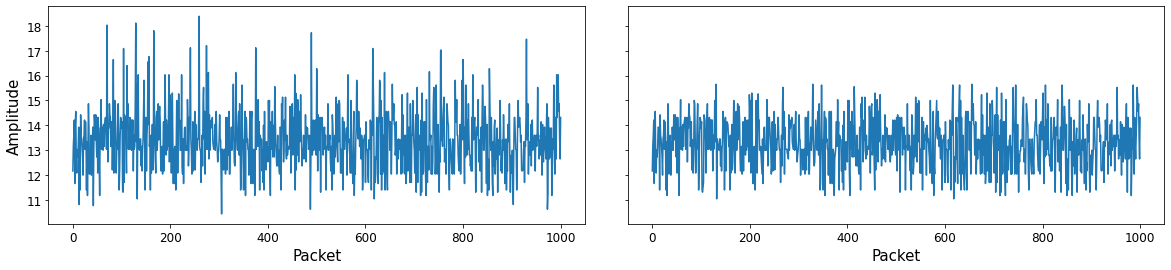
\includegraphics[width=0.98\textwidth]{images/Hampel1.png}
    \caption{Raw and filtered amplitudes of a single subcarrier over 10 seconds of acquisitions.}
    \label{fig:Hampel1}
\end{figure}
The detection procedure is performed independently on each subcarrier’s amplitude series, and every discovered outlier is substituted
with the mean of the previous and next non-outlier data point, to preserve temporal information consistency. Moreover, the Hampel Identifier
doesn't pose any assumption on the distribution of the data and works well even with non-normally distributed points. This is a clear distinction
with respect to other outlier detection statistical methods such as the Z-Score, that uses the mean and the standard deviation to discern anomalies
from the rest of the dataset. These measures assume that the data follows a symmetric Gaussian distribution, and they can be highly affected by skewness
or extreme outliers in case of non-normally distributed data. On the other hand, using the Median ensures resistance to skewness and to outliers with large
magnitude, and does not require any normality assumption.

\section{Phase Sanitization}
\bibliography{references}
\bibliographystyle{ieeetr}

\end{document}
